\documentclass{standalone}

\usepackage{tikz}
\usepackage{ifthen}
\usetikzlibrary{automata,positioning}

\begin{document}
	
	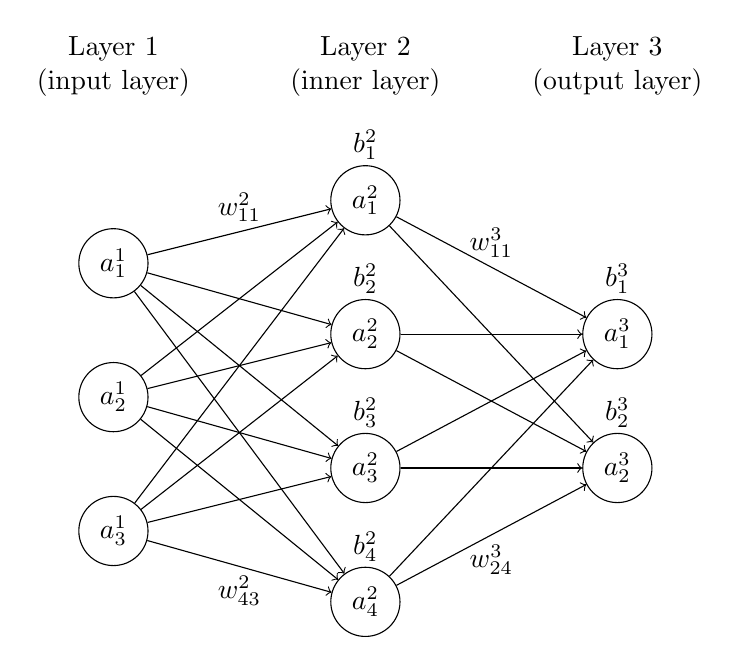
\begin{tikzpicture}[node distance=1.7cm,->]
		\node[align=center](l2){Layer 2\\(inner layer)};
		\node[state,below of=l2](12){$a_1^2$};
		\node[above of=12,yshift=-1cm](){$b_1^2$};
		\node[state,below of=12](22){$a_2^2$};
		\node[above of=22,yshift=-1cm](){$b_2^2$};
		\node[state,below of=22](32){$a_3^2$};
		\node[above of=32,yshift=-1cm](){$b_3^2$};
		\node[state,below of=32](42){$a_4^2$};
		\node[above of=42,yshift=-1cm](){$b_4^2$};
		
		\node[align=center,left of=l2,xshift=-1.5cm](l1){Layer 1\\(input layer)};
		\node[state,below of=l1,yshift=-.8cm](11){$a_1^1$};
		\node[state,below of=11](21){$a_2^1$};
		\node[state,below of=21](31){$a_3^1$};
		
		\node[align=center,right of=l2,xshift=1.5cm](l3){Layer 3\\(output layer)};
		\node[state,right of=22,xshift=1.5cm](13){$a_1^3$};
		\node[above of=13,yshift=-1cm](){$b_1^3$};
		\node[state,below of=13](23){$a_2^3$};
		\node[above of=23,yshift=-1cm](){$b_2^3$};
		 
		\foreach \i in {1,...,3} {
			\foreach \j in {1,...,4} {
				\ifthenelse{\i=1 \AND \j=1}
					{\draw (\i1) edge[above] node[align=center]{$w_{\j\i}^2$} (\j2);}
				{\ifthenelse{\i=3 \AND \j=4}
					{\draw (\i1) edge[below] node[align=center]{$w_{\j\i}^2$} (\j2);}
				{\draw (\i1) edge node {} (\j2);}}
						    
			}
		}
		
		\foreach \i in {1,...,4} {
			\foreach \j in {1,2} {
				\ifthenelse{\i=1 \AND \j=1}
					{\draw (\i2) edge[above] node[align=center]{$w_{\j\i}^3$} (\j3);}
				{\ifthenelse{\i=4 \AND \j=2}
					{\draw (\i2) edge[below] node[align=center]{$w_{\j\i}^3$} (\j3);}
				{\draw (\i2) edge node {} (\j3);}}
				
			}
		}
	\end{tikzpicture}
	
\end{document}